\documentclass[10pt,a4paper]{article}

\usepackage{enumerate}
\usepackage[top=2in, bottom=1.5in, left=1in, right=1in]{geometry}
\usepackage{fancyhdr} 		% page header
\usepackage{listings} 		% present source code.
\usepackage{amsmath}
\usepackage{amssymb}
\usepackage{float}
\usepackage{graphicx}
\usepackage{epstopdf}
\usepackage{hyperref}
\usepackage{lipsum}			% just to generate text for the example

\pagestyle{fancy} 
\fancyhf{}
\fancyhead[L]{CS 540-1}
\fancyhead[R]{Fall 2018}

\def\x{\mathbf{x}}
\def\y{\mathbf{y}}
\def\w{\mathbf{w}}
\def\p{\mathbf{p}}

\begin{document}
\begin{center}
{\bf \large CS 540-1: Introduction to Artificial Intelligence

Homework Assignment \# 2

\vspace{0.5cm}

Assigned:  9/13 

Due:  9/20 before class} 
\end{center}

\vspace{1cm}

\begin{center}
{\bf \Large Hand in your homework:}
\end{center}
This homework includes one written question and one programming question. Please type the written portion and hand in a pdf file named \textbf{hw2.pdf}. For the programming question, hand in the Java program \textbf{successor.java}. 
Go to UW Canvas, choose your CS540-1 course, choose Assignment, click on Homework 2: this is where you submit your files.




\section*{Problem 1. Search [60]}


Given the undirected, unweighted graph in Figure~\ref{fig:unweighted}, find the shortest path \textbf{from A to G} using different search algorithms. 

You are to ``run'' the algorithms by hand.  Use a CLOSED data structure to avoid cycles. Specifically, for uninformed search and uniform cost search follow slides 28 and 43 (Hint: these slides allow multiple copies of the same node in OPEN); for A* search follow slide 21. 

To break ties, assume nodes are expanded (taken out of the OPEN data structure) in alphabetical order with everything else being equal. 


For each algorithm, write down :
\vspace{-2mm}
\begin{itemize}
 \setlength{\topsep}{0pt}
 \setlength{\itemsep}{0pt}
 \setlength{\parskip}{0pt}
 \setlength{\parsep}{0pt}
 \item States of OPEN and CLOSED in each step of the algorithm, together with the appropriate back pointer (see example steps below)
 \item The solution path found
\end{itemize}

\begin{figure}[hb]
\centering
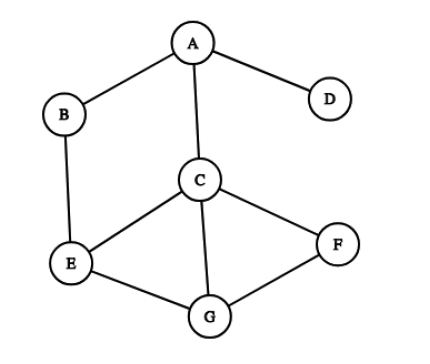
\includegraphics[width=0.5\textwidth]{graph.jpg}
\caption{The unweighted, undirected graph}
\label{fig:unweighted}
\end{figure}

\noindent a) [10] {Breadth First Search}.

The first few iterations of Breadth First Search have been shown to help you start.

\begin{center}
 \begin{tabular}{|l | l|} 
 \hline
 \textbf{OPEN (Queue)[Top is towards right]} & \textbf{CLOSED} \\  
 \hline
 A(Null) & \\
 \hline
 D(A), C(A), B(A) & A(Null)\\ 
 \hline
 E(B), A(B), D(A), C(A) & A(Null), B(A)\\
 \hline
 \dots & \dots \\
 \hline
\end{tabular}
\end{center}


\noindent b) [10] {Depth First Search}.

\noindent c) [10] {Iterative Deepening}.  
Let us use the following convention: for the first depth cutoff (the very first iteration of the outer loop) we will goal check A and also A's successors, but nothing further.


\clearpage
\noindent Now suppose we have different edge costs and heuristic function $h$ as in Figure~\ref{fig:weighted}. 

\begin{figure}[!h]
\centering
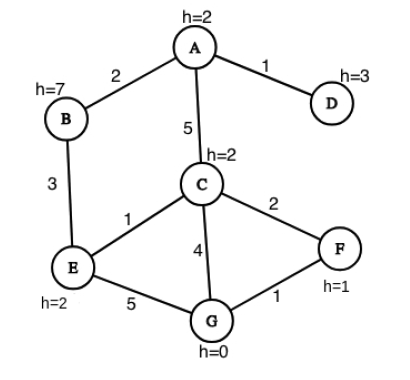
\includegraphics[width=0.5\textwidth]{graphc.png}
\caption{The weighted graph and the $h(\cdot)$ function}
\label{fig:weighted}
\end{figure}

For parts (d) and (e) also include the node score (for A* this is $g+h$) in your answer alongside with the back pointer. 

\noindent d) [10] Perform \textbf{Uniform Cost Search}.
The first few steps are shown for Uniform Cost Search in the example table below.
\begin{center}
\begin{tabular}{|l|l|}
\hline
\textbf{OPEN (Priority Queue)[Top is towards right]} & \textbf{CLOSED}\\
\hline
A(0,Null) & \\
\hline
C(5,A), B(2,A), D(1,A) & A(0,Null) \\
\hline
 \dots & \dots \\
 \hline
\end{tabular}
\end{center}



\noindent e) [20] Perform \textbf{A* search} with the given heuristic function $h(\cdot)$ in Figure~\ref{fig:weighted}.


\newpage

\section*{Problem 2. Successor Function [40]}
This is a programming question. The solution to the programming problem should be coded in Java, and
\textbf{you are required to use only built-in libraries} to complete this homework. Please submit a source code file named \textbf{successor.java} with \textbf{no package statements}, and make sure your program is runnable from command line on a department Linux machine. We provide a skeleton successor.java code that you can optionally use, or you can write your own. \\ \\
The goal of this assignment is to become familiar with the state space in a real-world problem. \\
You are given two water jugs with capacity A and B liters respectively. A and B are positive integers. At each step, you can perform one of these actions:
\begin{itemize}
 \setlength{\topsep}{0pt}
 \setlength{\itemsep}{0pt}
 \setlength{\parskip}{0pt}
 \setlength{\parsep}{0pt}
 \item Empty a jug
 \item Fill a jug
 \item Pour water from one jug to another until either the former is empty or the latter is full.
\end{itemize}

\noindent Write a program \textbf{successor.java} to print the successor states of an input state.
\begin{itemize}
 \setlength{\topsep}{0pt}
 \setlength{\itemsep}{0pt}
 \setlength{\parskip}{0pt}
 \setlength{\parsep}{0pt}
 \item Input: 4 integers $A, B, a, b$, where $(A, B)$ are the capacity of the jugs, and $(a, b)$ are the current amount of water in each jug.  You may assume that the input is valid, namely $a\le A, b\le B$, and $A, B$ are positive integers, and $a, b$ are non-negative integers.   
 \item Output: Print the list of successor states reachable in one step from $(a,b)$, one on each line.  The lines must be sorted as per the examples shown (using the provided sorting function in the skeleton code).  The successors should not include $(a,b)$ itself or duplicates.
\end{itemize}

Here are some examples of running the program from the command line.
The inputs and outputs are space-separated with no comma.
Please follow the same input/output format.

\noindent{Example 1:}
\begin{verbatim}
$java successor 3 2 3 1
0 1
2 2
3 0
3 2
\end{verbatim}

\noindent{Example 2:}
\begin{verbatim}
$java successor 11 5 6 3
0 3
4 5
6 0
6 5
9 0
11 3
\end{verbatim}

\end{document}
